% 黒魔術
\expandafter\ifx\csname ifdraft\endcsname\relax
    \documentclass[a4paper,twoside,12pt,papersize, dvipdfmx]{iirthesis}
    \usepackage{amsmath,amssymb,amsthm}
    \usepackage{graphicx}
    \usepackage{subcaption}
    \usepackage{url}
%    \usepackage{otf}
    \usepackage{minitoc}
    \usepackage{bm}
    \usepackage{amsmath,amssymb}
    \begin{document}

    \newcommand{\figref}[1]{\figurename\ref{#1}}
    \newcommand{\tabref}[1]{\tablename\ref{#1}}
    \renewcommand{\eqref}[1]{式~(\ref{#1})}
    \newcommand{\chapref}[1]{\ref{#1}章}
    \newcommand{\secref}[1]{\ref{#1}節}
    \newcommand{\ssecref}[1]{\ref{#1}項}
    \newcommand{\appref}[1]{付録\ref{#1}}
\fi


\chapter{平面内センサレスin-handケージングマニピュレーション}\label{chap::sicm}
\minitoc

\section{概要}
\cite{asamura2013}で,「センサレスin-handケージングマニピュレーション」という新たなマニピュレーション手法が提案された.これは,ロボットハンドの位置制御のみで対象物を拘束できる「ケージング」\cite{rimon1999}を基にしたマニピュレーション手法である.ケージングは,ロボットハンドと対象物の間の力のつり合いによって対象物を拘束する把持とは異なり,対象物の形状情報を基に幾何学的に囲い込むことで拘束する.そのため,力情報を必要としない.また,「囲い」による拘束であるため,対象物の詳細な位置情報も必要としない.一般的なIn-handマニピュレーション手法では,対象物の位置情報や力情報を必要とする.一方,本手法ではケージングを利用することにより,これらの情報を必要としない,センサレスなマニピュレーションが可能となっている.\par
本手法の特徴として,上述のセンサを必要としないことに加えて,外乱に強いといった点も挙げられる.センサレスin-handケージングマニピュレーションでは,マニピュレーション中は常に対象物のケージングが成立している.そのため,マニピュレーション中に対象物に外乱が加わり位置・姿勢に変化が生じても,最後までマニピュレーションを行うことができる.\par
本手法は,センサを用いていないため,動作計画において対象物の正確な位置・姿勢情報を使うことはできない.しかし,対象物の形状情報は既知であるため,ケージングが成立している任意のハンド姿勢による囲い内において,対象物が存在できる位置・姿勢群は算出できる.そこで,ケージングに関する条件を満たしながら,囲いの形状を変化させていく過程で,対象物が存在できる位置・姿勢群の数を十分に減らし,かつ目標位置・姿勢付近へと十分に近づけることで,センサレスに対象物を目標位置・姿勢へと位置決めすることができる.\par
以下の節では,より具体的な説明を行っていく.\secref{sec::sicm::partsfeeder}では,センサレスin-handケージングマニピュレーションを行うためのシステムの説明を行う.また,新たなハンド構成の提案についても記述する.\secref{sec::sicm::cspace}では,対象物の位置・姿勢群の扱い方について,\secref{sec::sicm::caging}では,センサレスin-handケージングマニピュレーションを可能とするためのケージングに関する条件について,\secref{sec::scim::planning}では,動作計画に使用しているアルゴリズムについて述べる.
%ケージングを用いることでセンサを必要としないこと
%オフラインで事前生成要素も書ければ書きたい

\section{汎用パーツフィーダ}\label{sec::sicm::partsfeeder}
センサレスin-handケージングマニピュレーションの位置・姿勢にばらつきのある対象物を特定の位置・姿勢に整列できるという機能を活かして,本手法はパーツフィーダへ応用することを見込んでいる.本研究では,ベルトコンベアと1対のロボットハンドを用いて\figref{}のように構成している.ロボットハンドは,3つのリンク,3つの関節からなる3自由度ハンドとなっている.ここで,\figref{}のように1対のロボットハンドを並列に並べたハンド構成を並列型ハンドと呼ぶこととする.
\subsection{一連の動作の流れ\cite{kamikukita2022}}\label{subsec::sicm::flow}
パーツフィーダの動作の流れについて説明する(\figref{}).まず,ハンドを開いた状態で,ベルトコンベアにより対象物を一定時間移動させ,停止する.その後,ハンドを閉じて物体を囲み,対象物のケージング状態を作った後にマニピュレーションを行う.整列が終了すると,ハンドを開いて物体を開放し,ベルトコンベアを一定時間動かして,対象物を流出させる.\par
本来のパーツフィーダでは,物体の分離と整列が必要となるが,本研究で扱うパーツフィーダは,物体の分離は行わず,ベルトコンベア上に十分な間隔で物体があることを前提として物体の整列動作を行う.
%上の\figref{}は全部同じ参照で,パーツフィーダの流れの説明した画像.上久木田卒論のFig3.2


\subsection{対向型ハンド}\label{subsec::sicm::oppositehand}
\ref{sec::intro::objective}で述べた通り,並列型ハンドでは対象物がハンド根元付近に詰まり,ハンドが正常に動けなくなるジャミング(\figref{})が発生していた.また,並列型ハンドの構造上,ハンド根元関節付近に対象物が存在する場合,マニピュレーションできないといった問題点も存在した.\par
そこで,\figref{}のようなハンド構成,対向型ハンドを提案する.
前者の問題に関して考える.%理論を考察する
後者の問題に関しては,一方のハンドの根元側に物体があったとしても,他方のハンドで掬い取るような動作でマニピュレーションできるため,解決が見込める.\par
対向型ハンドの弱点としては,横方向に大きく運べないという点が挙げられる.しかし,横方向の移動はベルトコンベアで賄えるので,大きな問題ではない.


\section{対象物のコンフィギュレーション空間}\label{sec::sicm::cspace}
本節では,ハンド動作計画の際に使用する,対象物のコンフィギュレーション空間について説明する.我々は対象物の状態を,位置$(x, y)$と姿勢(傾き)$\phi$の3変数によって表している.この3変数で構成される3次元空間が対象物のコンフィギュレーション空間である.空間内の任意の座標は,対象物の任意の位置・姿勢を表しており,それぞれ1:1に対応している.\par

このコンフィギュレーション空間の中から,対象物が存在できる領域を対象物のコンフィギュレーション自由空間と呼び,$C_{\mathrm{free}}$と表す.具体的な$C_{\mathrm{free}}$の導出は以下の通りである.まず,任意の座標$(x, y, \phi)$に対して,対象物の図心を$(x, y)$に合わせ,$\phi$だけ傾ける.このとき\figref{fig::sicm::cfree}(a)のようにハンドにも壁にも干渉しない場合,任意の座標$(x, y, \phi)$は$C_{\mathrm{free}}$を構成する点として認められ,\figref{fig::sicm::cfree}(b)のように干渉した場合は,$C_{\mathrm{free}}$を構成する点としては認めない.この判定を空間全体に対して行ったときの前者の集合が$C_{\mathrm{free}}$となる.\par

実装にあたり,対象物のコンフィギュレーション空間を\figref{fig::sicm::discretize}のように格子状に分割し,離散的に取り扱っている.本来,コンフィギュレーション空間は連続した空間である.そのため,格子点の幅を狭めれば狭めるほど実際の表現に近くなる.一方で,格子点幅を狭めすぎると格子点数が増え,その分計算負荷が大きくなる.したがって,マニピュレーションの動作計画に支障のない範囲で格子点幅を確保しつつ,計算負荷も抑えられるようなバランスの良いパラメータ設定が重要となる.\par

一例として,6自由度並列型ハンドで長方形物体をケージングした際の対象物コンフィギュレーション$C_{\mathrm{free}}$を\figref{fig::sicm::cfreeexam}に示す.この$C_{\mathrm{free}}$を評価することで,現在のハンド姿勢がセンサレスin-handケージングマニピュレーションするにあたって,妥当な姿勢か否かを判定する.この判定については,次節で説明する.



\begin{figure}[b]
\begin{minipage}{0.5\hsize}
\centering
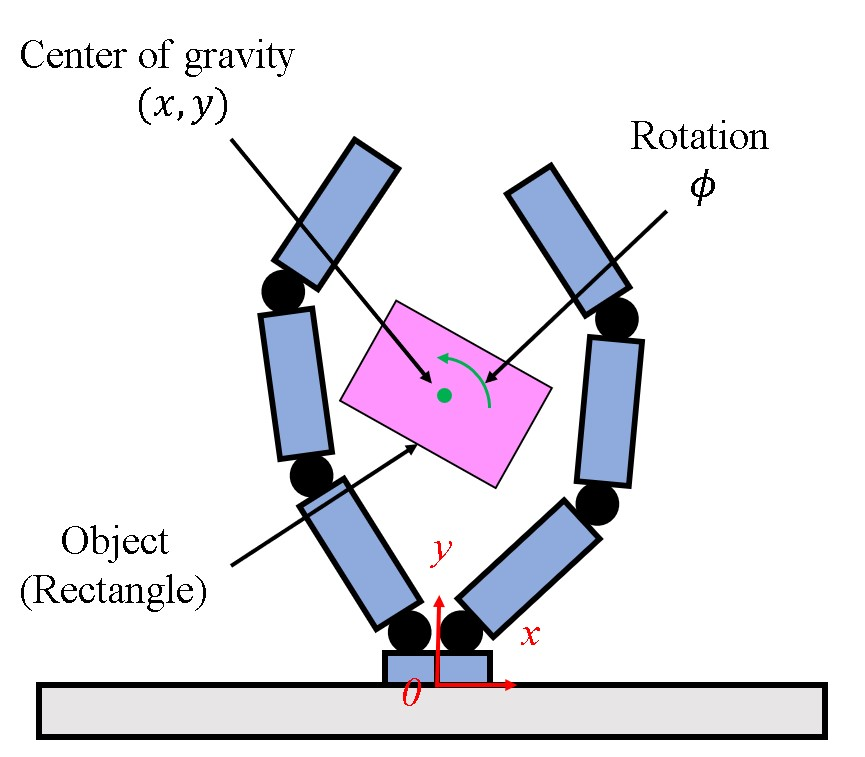
\includegraphics[width=0.9\hsize]{fig/Sensorless_ICM/define_cfree.jpg}
\end{minipage}
\begin{minipage}{0.5\hsize}
\centering
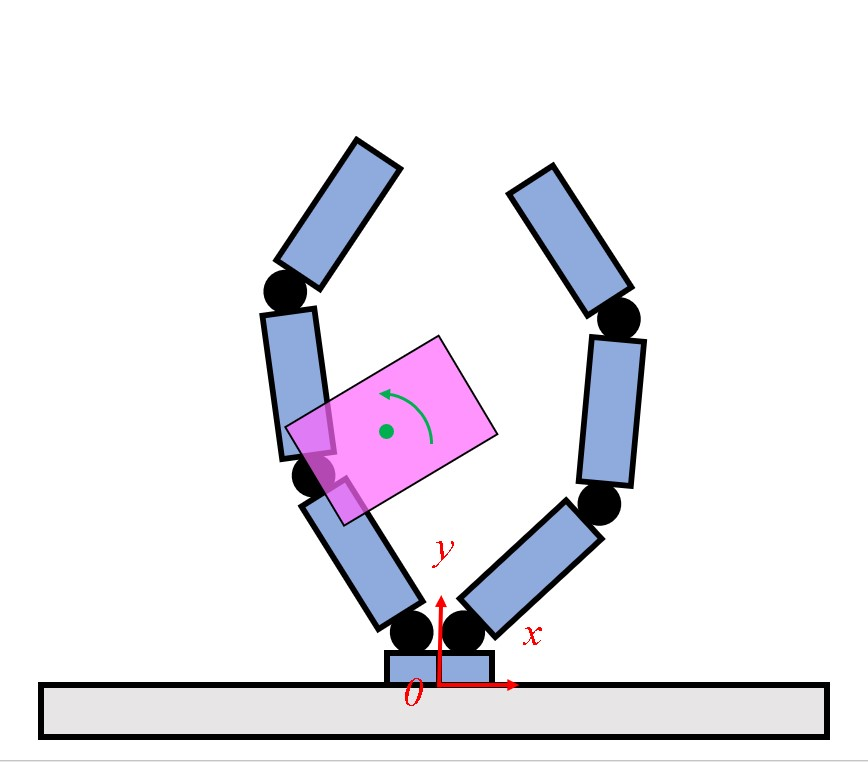
\includegraphics[width=0.9\hsize]{fig/Sensorless_ICM/define_notcfree.jpg}
\end{minipage}
\caption{Definition of $C_{\mathrm{free}}$}
\label{fig::sicm::cfree}
\end{figure}

%fig::sicm::discretizeは込山2020のFig.3.2
%fig::sicm::cfreeexamは込山2020のFig.3.4


\section{ケージング条件とケージングマニピュレーション可能条件}\label{sec::sicm::caging}
\subsection*{ケージング条件}
\cite{yokoi2010}よりケージング成立条件は以下のようになる.
ここで,次のように記号を定義する.
\begin{itemize}
\item $\mathcal{C}$: 物体のコンフィギュレーション空間
\item $\mathcal{A}_{\mathrm{obj}}$: 実空間での物体の領域
\item $\mathcal{A}_{\mathrm{finger}}$: 実空間でのロボットハンドの指部分の領域
\item $\mathcal{A}_{\mathrm{palm}}$: 実空間でのロボットハンドのパームの領域
\item $\bm{q}_{\mathrm{obj}}$: 物体のコンフィギュレーション
\item $\bm{q}_{\mathrm{fin}}$: ハンドの指部分のコンフィギュレーション
% \item $\bm{q}_{\mathrm{goal}}$: ハンドの指部分の目標コンフィギュレーション
\end{itemize}

まず,物体がハンドの指部分と接触するために進入することのできない領域,
コンフィギュレーション障害物領域$\mathcal{C}_{\mathrm{cls}\_\mathrm{finger}}$を考えると,次のように表される.
\begin{equation}
\mathcal{C}_{\mathrm{cls\_finger}} =
\{\bm{q}_{\mathrm{obj}} \in \mathcal{C} | \mathcal{A}_{\mathrm{obj}}(\bm{q}_{\mathrm{obj}})
\cap \mathcal{A}_{\mathrm{finger}}(\bm{q}_{\mathrm{finger}}) \not= \emptyset\}
\label{eq:obj-conf}
\end{equation}

同様に,物体とパームが干渉するために進入することのできない領域,
コンフィギュレーション障害物領域$\mathcal{C}_{\mathrm{cls\_palm}}$は次のように表される.
\begin{equation}
\mathcal{C}_{\mathrm{cls\_palm}} = \{\bm{q}_{\mathrm{obj}} \in \mathcal{C} | \mathcal{A}_{\mathrm{obj}}(\bm{q}_{\mathrm{obj}}) \cap \mathcal{A}_{\mathrm{palm}} \neq \emptyset\}
\label{eq:palm-conf}
\end{equation}

式(\ref{eq:obj-conf}),(\ref{eq:palm-conf})より,パームを考慮した場合でのコンフィギュレーション障害物領域は次のように表される.
\begin{equation}
\mathcal{C}_{\mathrm{cls}} = \mathcal{C}_{\mathrm{cls\_finger}} \cup  \mathcal{C}_{\mathrm{cls\_palm}}
\end{equation}

このとき,物体がハンドの指部分およびパームと干渉することなく取ることができるコンフィギュレーション領域を
$\mathcal{C}_{\mathrm{free}}$と定義する.$\mathcal{C}_{\mathrm{free}}$は,次のように表される.
\begin{equation}
\mathcal{C}_{\mathrm{free}} = \mathcal{C} \setminus  \mathcal{C}_{\mathrm{cls}}
 = \left(\mathcal{C} \setminus  \mathcal{C}_{\mathrm{cls\_finger}}\right) \setminus \mathcal{C}_{\mathrm{cls\_palm}}
\end{equation}

次に,$\bm{q}_{\mathrm{obj}}\not\in \mathcal{C}_{\mathrm{cls}}$を物体の初期コンフィギュレーションとしたとき,
物体が取り得るコンフィギュレーション領域$\mathcal{C}_{\mathrm{free\_obj}}$は次のように表される.
\begin{equation}
\mathcal{C}_{\mathrm{free\_obj}} = \{ \bm{q} \in \mathcal{C}_{\mathrm{free}} | \mathrm{connected} (\bm{q},\bm{q}_{\mathrm{obj}}) \}
\end{equation}

ここで,$\mathrm{connected} (\bm{q},\bm{q}_{\mathrm{obj}})$とは,
物体がコンフィギュレーション$\bm{q}_{\mathrm{obj}}$から$\bm{q}$へ,
障害物と干渉することなく移動可能であることを示す.

同様に,$\bm{q}_{\mathrm{inf}}\in \mathcal{C}$を無限遠点とすると,
無限点と繋がっているコンフィグレーション自由領域$\mathcal{C}_{\mathrm{free\_inf}}$は次のように表される.
\begin{equation}
\mathcal{C}_{\mathrm{free\_inf}} = \{ \bm{q} \in \mathcal{C}_{\mathrm{free}} | \mathrm{connected} (\bm{q},\bm{q}_{\mathrm{inf}}) \}
\end{equation}

ケージングが成立するための必要十分条件は,
物体が存在し得る領域が存在し,
かつ物体が無限遠へ移動不可能であることである(\figurename\ref{fig:c_free_obj_with_palm}).
よって,ケージング成立条件として,次の条件を満たす必要がある.
\begin{equation}
\begin{cases}
\mathcal{C}_{\mathrm{free\_obj}} \neq \emptyset \\
\mathcal{C}_{\mathrm{free\_obj}} \cap \mathcal{C}_{\mathrm{free\_inf}} = \emptyset
\end{cases}
\label{eq:object_closure}
\end{equation} 

% \begin{figure}[b]
% \centering
% \includegraphics[width=0.5\linewidth,clip]{fig/c_free_obj_with_palm.eps}
% \caption{Object Closure by Fingers and a Palm}
% \label{fig:c_free_obj_with_palm}
% \end{figure}


\subsection*{ケージングマニピュレーション可能条件}
\cite{yokoi2010}ではケージングマニピュレーションの可能条件として次の条件を挙げた.
\begin{itemize}
\item $\mathcal{C}_{\mathrm{free\_obj}}$が不連続に減少しない
% \item 環境のみによるObject Closure 状態ではない
\end{itemize}

ここで「不連続な減少」について説明する.
時間間隔$\Delta t$で考えることとして,\figurename\ref{fig:discontinuous_shrinkage}のように
時刻$t$から時刻$t+\Delta t$の間において,ロボットが連続的な移動をしていたとしても$\mathcal{C}_{\mathrm{free\_obj}}$が不連続な減少をする場合がある.
ケージングにおいては物体の位置を特定することができないため,$\mathcal{C}_{\mathrm{free\_obj}}$の不連続な減少が生じてその減少した領域内に物体が存在していた場合,
マニピュレーションを継続するには物体の不連続な移動が求められることになる.しかし,そのような移動は物理的に不可能である.
つまり,$\mathcal{C}_{\mathrm{free\_obj}}$の不連続な減少が生じた場合,
物体の位置によってはマニピュレーションが不可能となる.


また\figurename\ref{fig:split}のように$\mathcal{C}_{\mathrm{free\_obj}}$が分断されてしまった場合,どちらの領域に対象物が存在するか判定することができないが,
どちらに存在した場合でも分断された領域の片方が$\mathcal{C}_{\mathrm{free\_obj}}$でなくなるため$\mathcal{C}_{\mathrm{free\_obj}}$が不連続に減少したと見なせる.

よって,$\mathcal{C}_{\mathrm{free\_obj}}$が不連続な減少を生じた場合,マニピュレーション不可能と判定する.
なお,$\mathcal{C}_{\mathrm{free\_obj}}$の不連続な増加に関しては,
物体が存在し得る領域が大きくなるだけであるので,マニピュレーション可能条件において問題とはならない.
この条件は以下のように書くことができる.
\begin{equation}
\lim_{\Delta t \rightarrow +0} \bigl( \mathcal{C}_{\mathrm{free\_obj}}(t) \cap \mathcal{C}_{\mathrm{free\_obj}}(t+\Delta t) \bigr)
= \mathcal{C}_{\mathrm{free\_obj}}(t)
\label{eq:manipulability}
\end{equation}
式(\ref{eq:manipulability})は,左辺の極限が存在し,
なおかつ右辺と等しい場合,
時刻$t$から時刻$t + \Delta t$の間での$\mathcal{C}_{\mathrm{free\_obj}}$の減少が不連続でないことを意味する.

以上より摩擦のない理想的な状態では,式\eqref{eq:object_closure},\eqref{eq:manipulability}を満たす
ロボットハンドの経路を生成することができれば,対象物のセンシングをせずに,位置制御だけでこのIn-hand ケージングマニピュレーションが行うことができる.


\section{ハンドの動作計画}\label{sec::scim::planning}
%この従来アルゴリズムのデメリットも書く.




% 白魔術
\expandafter\ifx\csname ifdraft\endcsname\relax
    \end{document}
\fi
